\documentclass{standalone}
\usepackage{pgfplots}
\pgfplotsset{compat=1.18}

\begin{document}

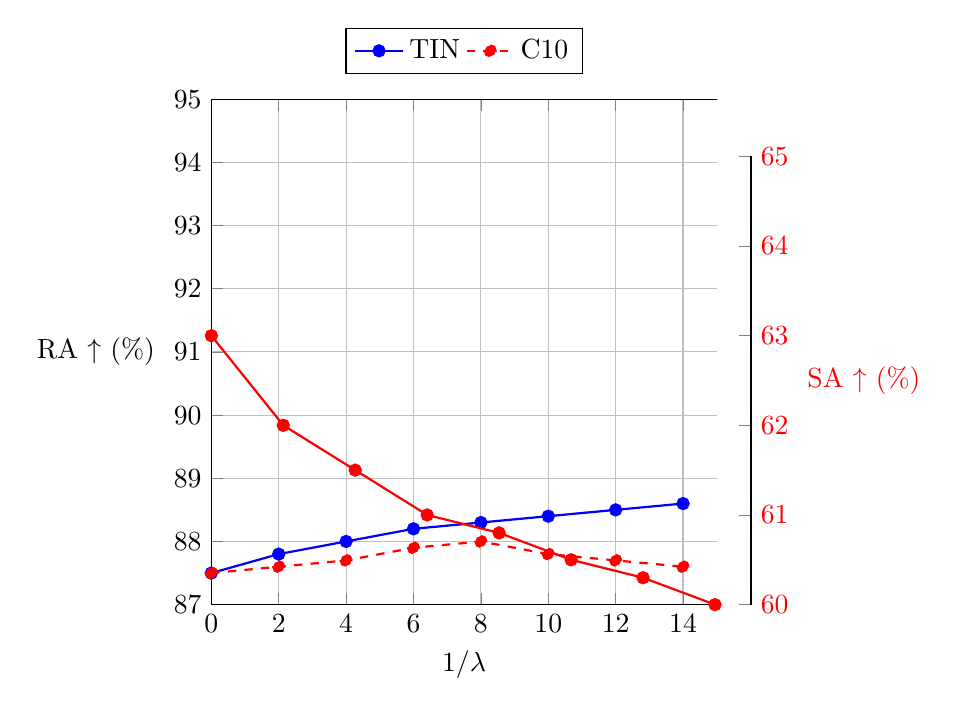
\begin{tikzpicture}
    \begin{axis}[
        width=8cm, height=8cm,
        xmin=0, xmax=15,
        ymin=87, ymax=95,
        ytick={87, 88, 89, 90, 91, 92, 93, 94, 95},
        yticklabels={87, 88, 89, 90, 91, 92, 93, 94, 95},
        axis y line*=left,
        xlabel={$1/\lambda$},
        ylabel style={rotate=-90},
        ylabel={RA $\uparrow$ (\%)},
        legend style={at={(0.5,1.05)},anchor=south,legend columns=2},
        legend cell align={left},
        grid=major,
        ]

        % Plot for RA
        \addplot[blue, thick, mark=*] coordinates {
            (0, 87.5) (2, 87.8) (4, 88.0) (6, 88.2) (8, 88.3) (10, 88.4) (12, 88.5) (14, 88.6)
        };
        \addlegendentry{TIN}

        \addplot[red, thick, dashed, mark=*] coordinates {
            (0, 87.5) (2, 87.6) (4, 87.7) (6, 87.9) (8, 88.0) (10, 87.8) (12, 87.7) (14, 87.6)
        };
        \addlegendentry{C10}

    \end{axis}

    \begin{axis}[
        xmin=0, xmax=15,
        ymin=60, ymax=65,
        ytick={60, 61, 62, 63, 64, 65},
        axis y line*=right,
        axis x line=none,
        ylabel style={rotate=-90},
        ylabel={SA $\uparrow$ (\%)},
        yticklabel style={red},
        ylabel style={red},
        ]

        % Dummy plot for the right y-axis (to scale correctly)
        \addplot[red, thick, mark=*] coordinates {
            (0, 63) (2, 62) (4, 61.5) (6, 61) (8, 60.8) (10, 60.5) (12, 60.3) (14, 60)
        };
    \end{axis}

\end{tikzpicture}

\end{document}